\chapter{Introduction}\label{chp:introduction}

Dengue is a mosquito-borne viral infection primarily transmitted by
\textit{Aedes aegypti} mosquitoes. The disease, caused by any of the four
distinct serotypes of the Dengue virus, poses a significant global public health
challenge~\citep{shepard:2016}. Environmental and ecological changes, such as
rising temperatures, increased urbanization, and changing precipitation
patterns, have expanded the range of \textit{Aedes aegypti}, contributing to the
greater geographic spread of Dengue. Since its emergence in the late
18\textsuperscript{th} century in Asia and the Pacific, Dengue has become
endemic in many regions, with approximately half of the world's population
currently living in areas at risk~\citep{fares:2015,negreiros-2020}. Factors
such as rapid population growth, unplanned urban development, inadequate
sanitation, and healthcare inequality play a central role in the persistence and
resurgence of dengue.

% In 2021, the Pan American Health Organization (PAHO) reported more than $1.3$
% million cases of arboviral diseases in the Americas, with Dengue alone
% accounting for $1.1$ million cases, approximately 89\% of the total. Despite
% occupying about 45\% of Latin America's landmass, Brazil contributed to more
% 60\% of Dengue cases in the region~\citep{BardachEtal2019}. In 2022, Brazil
% reported 2,363,490 Dengue cases, representing 84.11\% of global cases and
% 99.65\% of those in South America; 1,210,760 of these were laboratory confirmed.

In the last year, 2024, Brazil reported approximately $10.239.883$ cases of
Dengue, accounting for $78,62\%$ of the world's cases and $92,10\%$ of the South
American cases~\citep{BardachEtal2019}. Of the reported cases, $10.231.692$ were
confirmed in the laboratory, $8.191$ were classified as severe, and $6.161$
resulted in death. According to the epidemiological report of the Brazil Health
Departments up to April 20, 2024, more than 11 states and 465 cities declared a
state of emergency~\citep{health-dp-1}. By 28 February 2025, Brazil had reported
$662.224$ cases of Dengue, which represents $86.43\%$ of the World's cases.
Figure~\ref{fig:dengue_reported_cases_graphic} displays a graph that shows
the number of Dengue cases in the world, South America, and Brazil from 1980 to
2024.

\begin{figure}[h!]
	\centering
	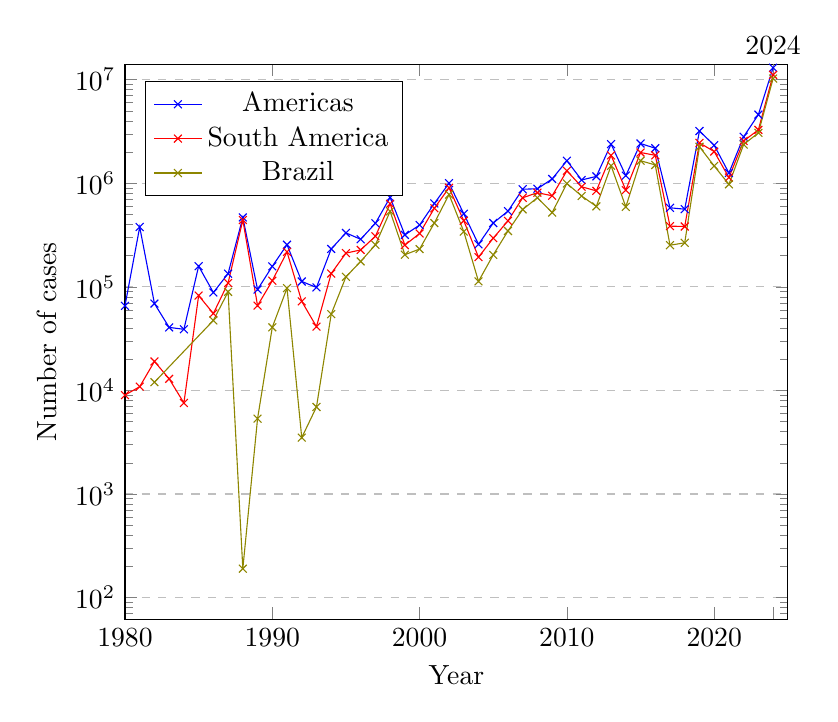
\begin{tikzpicture}[>=latex, scale=1]
		%scale=.6]
		\begin{axis}[
				width = {10cm},
				%title={Dengue reported cases from 1980 to 2022},
				xlabel={Year},
				ylabel={Number of cases},
				ymode=log,
				xmin=1980, xmax=2025,
				ymin=0, ymax=14000000,
				xtick={1980, 1990, 2000, 2010, 2020, 2024},
				xticklabels={1980, 1990, 2000, 2010, 2020},
				extra x ticks={2024},
				extra x tick labels={2024},  % Labels at top
				extra x tick style={ticklabel pos=upper},
				legend pos=north west,
				ymajorgrids=true,
				grid style=dashed,
			]

			\addplot[
				color=blue,
				mark=x,
			]
			plot coordinates {
					(1980, 65523)
					(1981, 377916)
					(1982, 68892)
					(1983, 40544)
					(1984, 38904)
					(1985, 158193)
					(1986, 88093)
					(1987, 134013)
					(1988, 467386)
					(1989, 94179)
					(1990, 157662)
					(1991, 254749)
					(1992, 112567)
					(1993, 98598)
					(1994, 232051)
					(1995, 331417)
					(1996, 287519)
					(1997, 410392)
					(1998, 729425)
					(1999, 317158)
					(2000, 394857)
					(2001, 636977)
					(2002, 1001073)
					(2003, 506726)
					(2004, 257251)
					(2005, 413122)
					(2006, 537412)
					(2007, 874750)
					(2008, 884334)
					(2009, 1099742)
					(2010, 1648569)
					(2011, 1073990)
					(2012, 1164366)
					(2013, 2384803)
					(2014, 1184045)
					(2015, 2416018)
					(2016, 2175409)
					(2017, 579027)
					(2018, 561689)
					(2019, 3190778)
					(2020, 2326115)
					(2021, 1254648)
					(2022, 2811433)
					(2023, 4594823)
					(2024, 13036652)
				};
			\addlegendentry{Americas}

			\addplot[
				color=red,
				mark=x,
			]
			plot coordinates {
					(1980, 9003)
					(1981, 10861)
					(1982, 19034)
					(1983, 12925)
					(1984, 7560)
					(1985, 82273)
					(1986, 55248)
					(1987, 108955)
					(1988, 441382)
					(1989, 65803)
					(1990, 114431)
					(1991, 217077)
					(1992, 72319)
					(1993, 41250)
					(1994, 134342)
					(1995, 211396)
					(1996, 226960)
					(1997, 307625)
					(1998, 632804)
					(1999, 252762)
					(2000, 326846)
					(2001, 572876)
					(2002, 903891)
					(2003, 434264)
					(2004, 193334)
					(2005, 294943)
					(2006, 432661)
					(2007, 724077)
					(2008, 810134)
					(2009, 756755)
					(2010, 1317801)
					(2011, 923793)
					(2012, 843840)
					(2013, 1857228)
					(2014, 857983)
					(2015, 1978921)
					(2016, 1860466)
					(2017, 385076)
					(2018, 382243)
					(2019, 2453060)
					(2020, 2021272)
					(2021, 1134555)
					(2022, 2558083)
					(2023, 3274879)
					(2024, 11118085)
				};
			\addlegendentry{South America}

			\addplot[
				color=olive,
				mark=x,
			]
			plot coordinates {
					(1980, 0)
					(1981, 0)
					(1982, 12000)
					(1983, 0)
					(1984, 0)
					(1985, 0)
					(1986, 47367)
					(1987, 89393)
					(1988, 190)
					(1989, 5334)
					(1990, 40642)
					(1991, 97209)
					(1992, 3501)
					(1993, 6915)
					(1994, 54453)
					(1995, 124775)
					(1996, 175749)
					(1997, 254074)
					(1998, 535283)
					(1999, 204131)
					(2000, 231412)
					(2001, 412388)
					(2002, 778037)
					(2003, 341189)
					(2004, 112851)
					(2005, 203356)
					(2006, 345922)
					(2007, 558413)
					(2008, 724427)
					(2009, 520660)
					(2010, 994158)
					(2011, 753487)
					(2012, 597450)
					(2013, 1473645)
					(2014, 591080)
					(2015, 1649008)
					(2016, 1500535)
					(2017, 252054)
					(2018, 265934)
					(2019, 2248570)
					(2020, 1467142)
					(2021, 975474)
					(2022, 2363490)
					(2023, 3064739)
					(2024, 10239883)
				};
			\addlegendentry{Brazil}
		\end{axis}
	\end{tikzpicture}
	\caption{Dengue reported cases from 1980 to 2024~\citep{paho-1}.}
	\label{fig:dengue_reported_cases_graphic}
\end{figure}

The disease imposes substantial social and economic burdens, affecting not only
the health and well-being of individuals but also the broader economic
productivity and healthcare system. The financial impact of Dengue in Brazil is
profound, for example, annual expenditures on Dengue prevention and control
exceed BRL $1.6$ billion~\citep{negreiros-2020}. The direct costs include
healthcare expenses for hospitalization, medical treatment, and public health
campaigns aimed at controlling mosquito populations~\citep{negreiros:2008}.
Indirect costs, such as lost productivity due to illness and the long-term
effects of severe Dengue cases, add to the financial strain. Moreover, the
social consequences are equally alarming, with communities enduring the
disruption of daily life, increased anxiety over disease outbreaks, and the loss
of lives.

Despite the severity of the situation, most Brazilian municipalities continue to
make crucial decisions in combating Dengue without the support of advanced
computational tools~\citep{brasil-dept-helth:2009}. The current approach is
largely reactive, relying on traditional mosquito control methods, including
eliminating adult mosquitoes, their breeding sites and public health
interventions. These actions are often insufficient to address the complexity
and scale of the problem. This lack of computational support means that
decisions regarding resource allocation, strategic planning, and the deployment
of interventions are not optimized, leading to possible inefficiencies and
potentially exacerbating the spread of the
disease~\citep{forbes-2002,xie-2015,rais-2011}.

The most common approach to combating Dengue spread is employing chemical
control methods, such as insecticides, which manage the mosquito population in
both the larval and adult stages~\citep{brasil-dept-helth:2009}. The \gls{who}
provides technical and operational standards for pesticide experts to ensure the
safe use of insecticides in public health. These standards specify the active
ingredients and dosages for various treatments. During disease outbreaks,
emergency responses in urban areas usually involve the dispatch of spraying
vehicles to apply insecticides (see Figure~\ref{fig:nebulizer}). It is essential
to use insecticides carefully and responsibly in vector control activities, as
indiscriminate use can have significant environmental impacts and contribute to
developing resistance in mosquitoes~\citep{WHO2009,WHO2020}.

\begin{figure}[h!]
	\centering
	\includegraphics[scale=0.5]{images/fumace.jpg}
	\caption{Nebulizer equipment attached to vehicle \citep{fumace-2022}.}
	\label{fig:nebulizer}
\end{figure}

The sprayed insecticide has no residual  effect and it is strongly influenced by
wind  and obstacles  along the  streets. The  best effect  is achieved  when the
densest  insecticide cloud  is at  a distance  of at  most 100  meters from  the
equipment~\citep{brasil-dept-helth:2009}.  As this  distance  is  crossed, the
effectiveness  decreases, as a consequence of droplet drift influenced by
factors of the environment. The cloud dispersion is illustrated in
Figure~\ref{fig:dispersion}.

\begin{figure}[!ht]
	\centering
	\includegraphics[scale=0.4]{images/cloud-dispersion.png}
	\caption{Cloud dispersion of the application \citep{brasil-dept-helth:2009}.}
	\label{fig:dispersion}
\end{figure}

Insecticide application instructions are generally based on ideal topology
conditions, locality structure, and favorable winds. The operation is often
affected by unpaved roads, the presence of high walls,  and  high   vegetation,
in  addition  to   headwinds.  The application methodology must consider these
limitations to obtain a good impact on the vector population. Once a spraying
vehicle begins to service a city block, it must sequentially cover all
surrounding streets in a clockwise direction. The traversal ensures that the
insecticide fog forms a continuous barrier, preventing mosquitoes from escaping.
The clockwise direction is due to real operational factors, as the nebulizer
equipment points to the right side of the vehicle.

Figure~\ref{fig:instance_digraph_fumace_car} shows an example of a map, with
four blocks to service, and Figure~\ref{fig:route_fumace_car} presents a
spraying route for these blocks where the nebulizer is activated in the black
dots and follows the direction of the arrow, starts by serving Block 2, goes to
Blocks 1, 3 and 4, respectively.

\begin{figure}[!ht]
	\begin{minipage}[c]{.49\textwidth}
		\centering
		\subfloat[Street blocks example.]{\label{fig:instance_digraph_fumace_car}\includegraphics[width=5cm, height=5cm]{images/cbrp-instance.pdf}} \end{minipage}%
	\begin{minipage}[c]{.49\textwidth}
		\centering
		\subfloat[Spraying route example.]{\label{fig:route_fumace_car}\includegraphics[width=8cm, height=5cm]{images/nebulizer-activated.pdf}}
	\end{minipage}
	\caption{Vehicle pattern with nebulizer \cite{brasil-dept-helth:2009}.}
\end{figure}

As a result, health authorities with limited budgets must make two key
decisions: first, selecting which city blocks should receive insecticide
spraying to maximize vector suppression; and second, optimizing vehicle routes
to ensure the efficient use of available resources. In this context, there is a
clear and urgent need to integrate computational models and decision-support
systems into Dengue control strategies. Such tools can help municipalities
better predict outbreaks, optimize resource use, and implement more effective
mosquito control measures.

In operations research, routing problems are typically classified based on where
the service is performed. When services are provided at specific locations
(nodes), they fall under \gls{vrp}~\citep{braekers2016vehicle}. When services
are conducted along edges (or arcs), they are categorized as
\gls{arp}~\citep{corberan2021arc}. The routing challenge in Dengue control
exhibits the characteristics of both \gls{vrp} and \gls{arp}. Each city block
can be represented as a \textit{super-node} (similar to a \gls{vrp}), while
spraying occurs along the surrounding arcs, aligning with \gls{arp} features.
Given this hybrid structure, we introduce and explore a new problem, titled the
\gls{cbrp}.

The \gls{cbrp} aims to optimize the servicing of city blocks within an urban
street network by assigning spraying vehicles. However, due to limited
operational resources, only a subset of city blocks can be serviced. A city
block is considered serviced if a spraying vehicle completely encircles it
without detours, and each serviced block contributes a predefined benefit. Thus,
the primary objective of the \gls{cbrp} is to identify the subset of blocks
whose servicing yields the highest aggregate benefit, alongside determining the
optimal vehicle routes to achieve this objective within the available resources.

The Figure~\ref{fig:ex1} illustrates an example of an input graph (city map) and
a corresponding \gls{cbrp} feasible solution. In Figure~\ref{subfig:a}, the
circles represent the graph nodes, while the labels from A to H indicate the
city blocks. Figure~\ref{subfig:b} depicts a feasible solution to the
\gls{cbrp}. In this solution, the nodes used in the route are marked as squares
and connected by black arrows (nodes 4, 5, 3, and 9). Squares with a double
border denote nodes that act as starting points to serve at least one block. The
atended blocks are represented by the arcs connected to the double square with
the same color, for example: node 4 (blue) serves blocks A (arcs
4$\rightarrow$8, 8$\rightarrow$1 and 1$\rightarrow$4) and B (arcs
4$\rightarrow$6, 6$\rightarrow$8 and 8$\rightarrow$4). Node 5 (red) serves
blocks D and F, node 3 does not serve any block, and node 9 (teal) serves block
H.

\begin{figure}[!ht]
	\begin{subfigure}{.5\textwidth}
		\begin{tikzpicture}[
				> = stealth, % arrow head style
				shorten > = 0.8pt, % don't touch arrow head to node
				auto,
				node distance = 1cm, % distance between nodes
				semithick % line style
			]

			\tikzstyle{every state}=[
			draw = black,
			thick,
			fill = white,
			minimum size = 5mm
			]

			\node[state] (a) [at={(-1, -0.5)}]{$1$};
			\node[state] (b) [at={(2,1.3)}] {$2$};
			\node[state] (c) [at={(4.5,1.3)}] {$3$};
			\node[state] (d) [at={(0.5, 0.5)}] {$4$};
			\node[state] (e) [at={(3, 0)}] {$5$};
			\node[state] (f) [at={(2,-1.5)}] {$6$};
			\node[state] (g) [at={(4,-1.5)}] {$7$};
			\node[state] (i) [at={(0.5,-1.5)}] {$8$};
			\node[state] (j) [at={(5,0)}] {$9$};
			\node[state] (k) [at={(5.5,-1.5)}] {$10$};
			% Blocks
			\node[state, draw = white, right of = a] {A};
			\node[state, draw = white, right of = i, yshift=0.8cm, xshift=-0.5cm] {B};
			\node[state, draw = white, below of = b, yshift=0.2cm] {C};
			\node[state, draw = white, left of = e, yshift=-0.4cm] {D};
			\node[state, draw = white, below of = e] {E};
			\node[state, draw = white, right of = b, yshift=-0.5cm] {F};
			\node[state, draw = white, right of = e] {G};
			\node[state, draw = white, below of = j, xshift=-0.2cm] {H};


			\path[->] (a) edge node {} (d);
			\path[->] (d) edge node {} (a);
			\path[->] (i) edge node {} (a);
			\path[->] (a) edge node {} (i);
			\path[->] (b) edge node {} (d);
			\path[->] (d) edge node {} (b);
			\path[->] (b) edge node {} (c);
			\path[->] (c) edge node {} (b);
			\path[->] (c) edge node {} (e);
			\path[->] (e) edge node {} (c);
			\path[->] (e) edge node {} (f);
			\path[->] (f) edge node {} (e);
			\path[->] (d) edge node {} (i);
			\path[->] (i) edge node {} (d);
			\path[->] (d) edge node {} (e);
			\path[->] (e) edge node {} (d);
			\path[->] (d) edge node {} (f);
			\path[->] (f) edge node {} (d);
			\path[->] (e) edge node {} (g);
			\path[->] (g) edge node {} (e);
			\path[->] (c) edge node {} (j);
			\path[->] (j) edge node {} (c);
			\path[->] (i) edge node {} (f);
			\path[->] (f) edge node {} (i);
			\path[->] (j) edge node {} (k);
			\path[->] (k) edge node {} (j);
			\path[->] (j) edge node {} (g);
			\path[->] (g) edge node {} (j);
			\path[->] (e) edge node {} (b);
			\path[->] (b) edge node {} (e);
			\path[->] (f) edge node {} (g);
			\path[->] (g) edge node {} (f);
			\path[->] (g) edge node {} (k);
			\path[->] (k) edge node {} (g);

		\end{tikzpicture}
		\subcaption{\label{subfig:a} Initial graph and blocks.}
	\end{subfigure}
	% Segunda figura
	\begin{subfigure}{.5\textwidth}
		\begin{tikzpicture}[
				> = stealth, % arrow head style
				shorten > = 0.8pt, % don't touch arrow head to node
				auto,
				node distance = 1cm, % distance between nodes
				semithick % line style
			]

			\tikzstyle{every state}=[
			draw = black,
			thick,
			fill = white,
			minimum size = 6mm
			]

			\node[state] (a) [at={(-1, -0.5)}]{$1$};
			\node[state] (b) [at={(2,1.3)}] {$2$};
			\node[state, rectangle] (c) [at={(4.5,1.3)}] {$3$};
			\node[state, rectangle, double, draw=blue] (d) [at={(0.5, 0.5)}] {$4$};
			\node[state, rectangle, double, draw=red] (e) [at={(3, 0)}] {$5$};
			\node[state] (f) [at={(2,-1.5)}] {$6$};
			\node[state] (g) [at={(4,-1.5)}] {$7$};
			\node[state] (i) [at={(0.5,-1.5)}] {$8$};
			\node[state, rectangle, double, draw=teal] (j) [at={(5,0)}] {$9$};
			\node[state] (k) [at={(5.5,-1.5)}] {$10$};
			% Blocks
			\node[state, thick, dashed, draw = white, right of = a] {A};
			\node[state, thick, dashed, draw = white, right of = i, yshift=0.8cm, xshift=-0.5cm] {B};
			\node[state, draw = white, below of = b, yshift=0.2cm] {C};
			\node[state, thick, dashed, draw = white, left of = e, yshift=-0.4cm] {D};
			\node[state, draw = white, below of = e] {E};
			\node[state, thick, dashed, draw = white, right of = b, yshift=-0.5cm] {F};
			\node[state, draw = white, right of = e] {G};
			\node[state, thick, dashed, draw = white, below of = j, xshift=-0.2cm] {H};
			% Dummy
			%\node[state, double, above of = a] (s) {s};
			%\node[state, double, right of = j, xshift=0.2cm] (t) {t};
			%\path[->, draw = black, opacity = 1.0] (s) edge node {} (d);
			%\path[->, draw = black, opacity = 1.0] (j) edge node {} (t);

			\path[->, draw = blue, opacity = 1.0] (a) edge node {} (d);
			\path[->, draw = gray, opacity = 0.1] (d) edge node {} (a);
			\path[->, draw = blue, opacity = 1.0] (i) edge node {} (a);
			\path[->, draw = gray, opacity = 0.1] (a) edge node {} (i);
			\path[->, draw = gray, opacity = 0.1] (b) edge node {} (d);
			\path[->, draw = gray, opacity = 0.1] (d) edge node {} (b);
			\path[->, draw = red, opacity = 1.0] (b) edge node {} (c);
			\path[->, draw = gray, opacity = 0.1] (c) edge node {} (b);
			\path[->, draw = red, opacity = 1.0, bend left=10] (c) edge node {} (e);
			\path[->, draw = black, opacity = 1.0, bend left=10, line width=0.5mm] (e) edge node {} (c);
			\path[->, draw = red, opacity = 1.0, bend right=10] (e) edge node {} (f);
			\path[->, draw = gray, opacity = 0.1] (f) edge node {} (e);
			\path[->, draw = blue, opacity = 1.0, bend right=10] (d) edge node {} (i);
			\path[->, draw = blue, opacity = 1.0, bend right=10] (i) edge node {} (d);
			\path[->, draw = black, opacity = 1.0, bend left=10, line width=0.5mm] (d) edge node {} (e);
			\path[->, draw = red, opacity = 1.0, bend right=10] (d) edge node {} (e);
			\path[->, draw = gray, opacity = 0.1] (e) edge node {} (d);
			\path[->, draw = blue, opacity = 1.0, bend right=10] (d) edge node {} (f);
			\path[->, draw = red, opacity = 1.0, bend right=10] (f) edge node {} (d);
			\path[->, draw = gray, opacity = 0.1] (e) edge node {} (g);
			\path[->, draw = gray, opacity = 0.1] (g) edge node {} (e);
			\path[->, draw = black, opacity = 1.0, line width=0.5mm] (c) edge node {} (j);
			\path[->, draw = gray, opacity = 0.1] (j) edge node {} (c);
			\path[->, draw = gray, opacity = 0.1] (i) edge node {} (f);
			\path[->, draw = blue, opacity = 1.0] (f) edge node {} (i);
			\path[->, draw = teal, opacity = 1.0] (j) edge node {} (k);
			\path[->, draw = gray, opacity = 0.1] (k) edge node {} (j);
			\path[->, draw = gray, opacity = 0.1] (j) edge node {} (g);
			\path[->, draw = gray, opacity = 0.1] (g) edge node {} (j);
			\path[->, draw = red, opacity = 1.0] (e) edge node {} (b);
			\path[->, draw = gray, opacity = 0.1] (b) edge node {} (e);
			\path[->, draw = gray, opacity = 0.1] (f) edge node {} (g);
			\path[->, draw = gray, opacity = 0.1] (g) edge node {} (f);
			\path[->, draw = gray, opacity = 0.1] (g) edge node {} (k);
			\path[->, draw = teal, opacity = 1.0] (k) edge node {} (g);
			\path[->, draw = teal, opacity = 1.0] (g) edge node {} (j);
		\end{tikzpicture}
		\subcaption{\label{subfig:b} Route and attended blocks.}
	\end{subfigure}
	\caption{\label{fig:ex1} CBRP instance (a) and solution (b).}
\end{figure}

Given the complex and dynamic nature of urban environments, particularly in
public health scenarios like Dengue control, incorporating stochastic elements
into the \gls{cbrp} is essential to enhance the realism and applicability of the
solution. Some unpredictable behavior of mosquitoes and the spread of Dengue
cases during seasons of the years highlight the need for a stochastic version of
the \gls{cbrp}. This leads to solutions that better reflect the variability of
actual deployment scenarios, improving the adherence of the model to real-world
challenges. Moreover, by accounting for probabilistic factors, stochastic
approaches can prioritize the most critical city blocks under uncertain resource
availability, thereby increasing the effectiveness and resilience of vector
control interventions.

The \gls{cbrp} extends beyond its application in vector control, providing a
robust framework to address a variety of urban logistics challenges. These
challenges include waste collection, postal delivery, and reading of utility
meters, where the primary goal is to efficiently service city blocks while
managing both spatial and resource constraints. The flexibility of the
\gls{cbrp} makes it particularly valuable in densely populated urban
environments, where the efficiency of routing decisions significantly affects
both service effectiveness and operational costs.

Besides the definition of control actions~\citep{gomez-2009,jing2019dengue}, it
is important to develop visualization and decision support tools to assist the
health departments. A clear understanding of the likely progression of Dengue
cases can significantly enhance short-term resource allocation
strategies~\citep{brasil-dept-helth:2009}. Generating accurate predictive models
for Dengue spread, especially in urban areas is highly challenging since
mosquito behavior is inconsistent and depends on numerous factors. These include
the availability and location of breeding sites, the mosquito population size
and infection rate, the timing and location of insecticide application,
frequency of rainfall, various climate conditions, and the interactions between
mosquitoes, breeding sites, and human populations.

In this thesis, we developed a complete set of methodologies focused in the
application of \gls{cbrp} to optimize insecticide-spraying routes for Dengue
control. Those methodologies compreend exact and heuristic approaches for
deterministic and stochastic versions of the \gls{cbrp}, instances based on real
data, robust simulation based on multi-agent systems and a
simulation-optimization framework that could assist health departments. This
application is particularly pertinent to many Brazilian cities, where seasonal
outbreaks of mosquito-borne diseases demand resource-efficient, targeted vector
control strategies. By optimizing spray routes, the \gls{cbrp} not only improves
operational efficiency but also maximizes coverage of high-risk areas,
ultimately supporting public health initiatives aimed at reducing Dengue
transmission.

% The \gls{mabs} have become increasingly popular in various fields due to their
% ability to capture the complexity and dynamics of real-world
% systems~\citep{siebers-2008}. Unlike traditional simulations that rely on a set
% of predetermined rules and assumptions, multi-agent simulations allow for
% interactions between agents to emerge organically, leading to the emergence of
% unexpected and emergent behaviors. This makes them an effective tool for
% understanding and predicting the behavior of complex systems, such as social and
% economic systems, ecological systems, and even biological
% systems~\citep{ballet-2020}. Additionally, multi-agent simulations provide a
% flexible and adaptable approach that can be easily modified and scaled to
% simulate different scenarios and environments. With the increasing availability
% of computing resources, multi-agent simulations have become an important tool
% for modeling and simulating complex systems, providing valuable insights into
% the behavior and evolution of these systems~\citep{selvaratnam-1995}.


%\paragraph{Our contributions.} The contributions of this study are three-fold.
% First, it advances vector control strategies by proposing novel methodologies
% for the optimal routing of spraying vehicles. Our approaches are based on
% mixed-integer linear programming (MILP) formulations and biased-random key
% genetic algorithms (BRKGA). Second, we introduce a systematic procedure for
% generating realistic problem instances by mapping city blocks and their
% surrounding street arcs. Third, through extensive computational experiments
% utilizing seven years of Dengue case data from two Brazilian cities, we
% demonstrate that our proposed methodologies significantly improve vector
% control effectiveness, potentially reducing Dengue transmission rates and
% improving public health outcomes. These findings offer valuable insights to
% public health authorities, policymakers, and researchers working on complex
% vector-borne disease challenges. Moreover, the generality of the CBRP
% framework makes it a promising approach for optimizing vehicle routing
% strategies in other city-block service applications.

% \paragraph{Text organization.}
% The remainder of this thesis is organized as follows.
% Chapter~\ref{chp:preliminary-concepts} formally defines the City Block Routing Problem (CBRP).
% Chapter~\ref{chp:literature_review} reviews existing operations research, \gls{ml} and simulation approaches relevant to Dengue vector control.
% Section~\ref{sec:models} introduces and describes the proposed mathematical formulations for the CBRP.
% Section~\ref{sec:data} explains the datasets and experimental setups employed to evaluate the proposed methodologies.
% Section~\ref{sec:results} discusses computational results and assesses the methodologies' performance.
% Finally, Section~\ref{sec:conclusions} summarizes the findings and provides concluding remarks.